\graphicspath{{./assets/}}
\setcounter{mtc}{8}
\chapter{6th Sprint: Deployment of the CI/CD platform }
\fancyhead[R]{\ungaramond\small\textbf{Chapter VIII.  6th Sprint:  Deployment of the CI/CD platform }}

\minitoc
\newpage
\section*{Introduction}
Deploying a CI/CD platform is essential for modern software development as it enables developers to automate and streamline the software development lifecycle from code to production. 

In this chapter, we will discuss the process of deploying a comprehensive CI/CD platform that contains Jenkins as a CI/CD orchestrator, a SonarQube cluster for code quality and ArgoCD for continuous deployment. 

Firstly, we will go over the sprint backlog for this chapter. 

Then, we will provide an overview of the different tools and technologies that will be used in this chapter, including Jenkins, SonarQube, ArgoCD and other tools. 

Lastly, we will cover the step-by-step process of deploying the CI/CD platform. 

\section{Sprint backlog :}

\begin{longtable}[H]{|m{1.5cm}|m{3cm}|m{1.5cm}|m{9cm}|}
\hline
{\textbf{Epic ID}} & {\textbf{Epic}} & {\textbf{Story ID}} & {\textbf{Story}}\\
\hline
1  & Self-hosting the ci/cd platform tools.  &  1.1	 & Setting up the CI/CD orchestrator.\\
\cline{3-4}
& & 1.2 & Setting up the container image builder. \\
\cline{3-4}
& & 1.3	& Setting up the code quality gate. \\
\cline{3-4}
& & 1.4	& Setting up the continuous delivery controller. \\
\cline{3-4}
\hline
\caption{6th Sprint Backlog}
\end{longtable}

\section{UML design: deployment diagram for the CI/CD platform} 

The following figure illustrates the deployment diagram for the CI/CD platform we put in place to: 
\begin{enumerate}[label = (\arabic*)]
\item automate builds, tests, and deployment processes. 
\item ensure code quality. 
\end{enumerate}

\begin{figure}[H]\centering
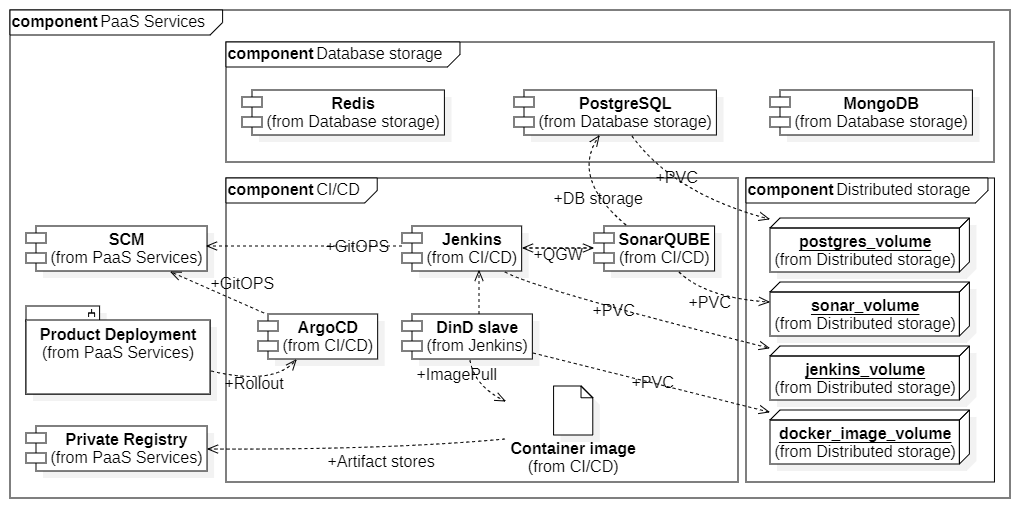
\includegraphics[width=1.0\textwidth,angle=00]{assets/f34.png}
\caption{deployment diagram for the CI/CD platform }
\label{fig:deployment diagram for the CI/CD platform}
\end{figure}

\section{Components of the CI/CD platform }

\subsection{The database storage backend }

When deploying databases like PostgreSQL, Redis, and MongoDB on Kubernetes, it is important to consider high availability and scalability as critical factors. 

\subsubsection{Activity diagram for deploying the database storage backend }
\begin{figure}[H]\centering
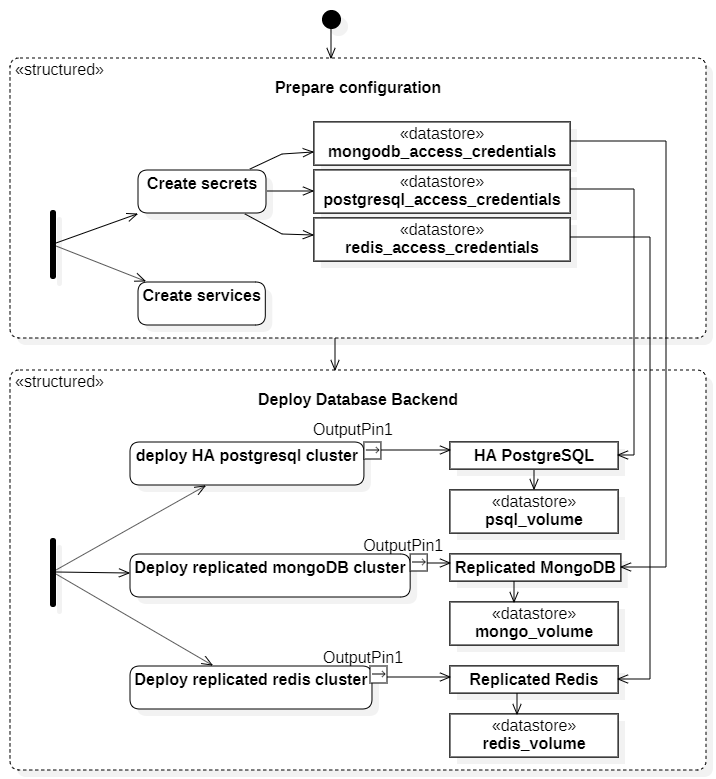
\includegraphics[width=1.0\textwidth,angle=00]{assets/f35.png}
\caption{Activity diagram for deploying the database storage backend}
\label{fig:Activity diagram for deploying the database storage backend}
\end{figure}

\subsubsection{Replicated MongoDB }

MongoDB is a popular NoSQL database that supports horizontal scaling through sharding and replication. To deploy a replicated mongodb cluster on Kubernetes, we used the following : 
\begin{itemize}[label={--}]
\item A secret that contains access credentials as well as a replica set key. 
\item Various configmaps that contain scripts for initializing the database server as well as its replicas. 
\item A statefulset for the arbiter which is a special type of node that does not store any data but participates in the election of a new primary node if the current primary node fails. 
\item A statefulset for mongodb which is configured to use environment variables as well as attachments from the created configmaps and secrets. 
\item The persistent volumes for storing data are provisioned using PersistentVolumeClaimTemplates in the statefulset. This ensures that data is preserved even if a MongoDB pod is terminated or rescheduled. 
\item A ClusterIP service for the mongodb arbiter (internal access only). 
\item NodePort services for each mongodb instance (both internal and external access to each node). 
\item A headless service (no IP) for the whole replicaSet (internal access). 
\item A LoadBalancer service for the mongodb primary instance (external access). 
\end{itemize}

Using a Kubernetes StatefulSet, we deployed multiple MongoDB instances in a replicated configuration and configured MongoDB replication for data synchronization. The following figure illustrates the workloads put in place: 


\begin{figure}[H]\centering
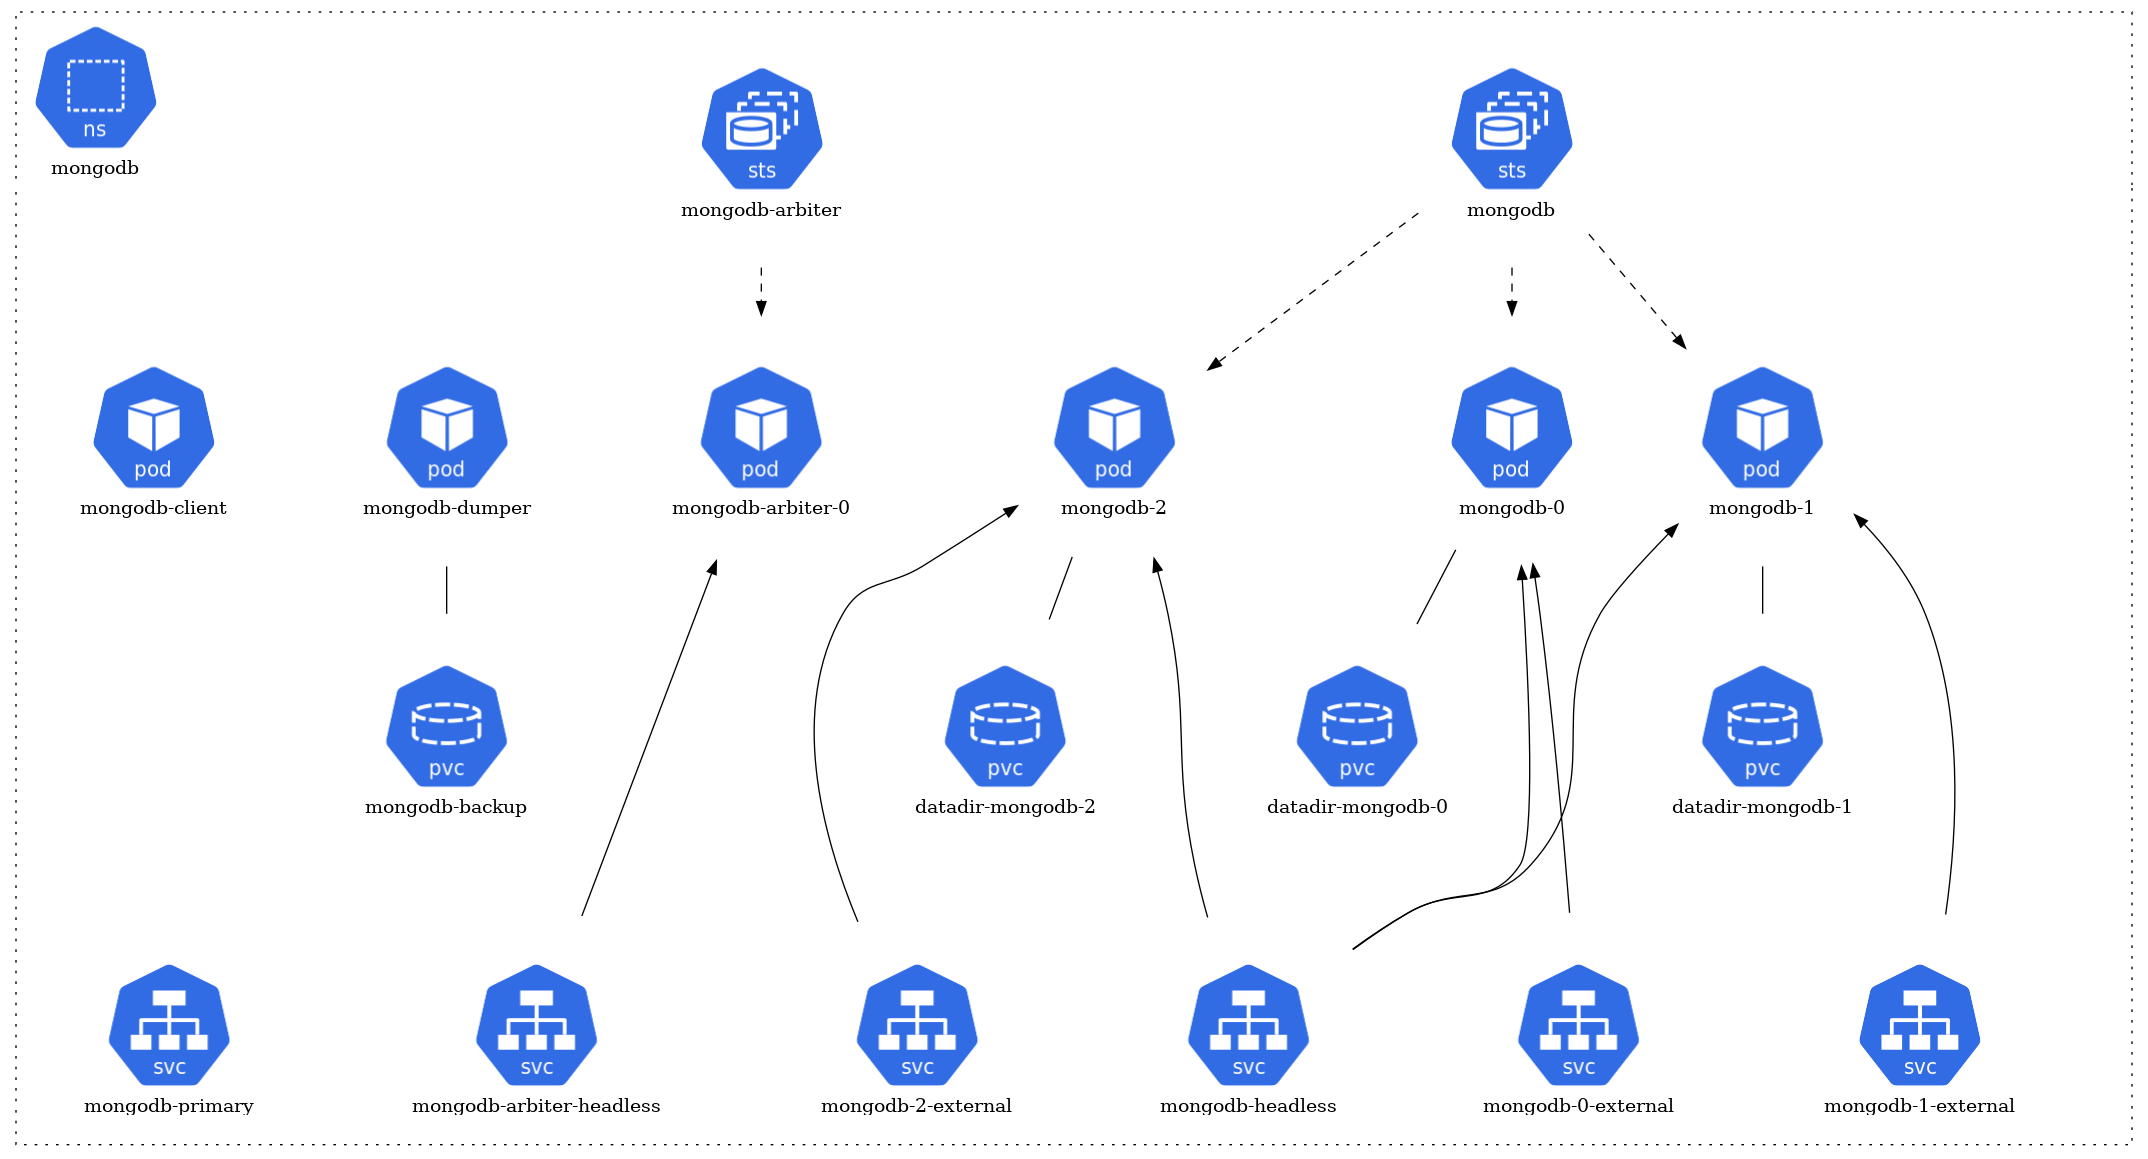
\includegraphics[width=1.0\textwidth,angle=00]{assets/f36.png}
\caption{MongoDB Workloads }
\label{fig:MongoDB Workloads}
\end{figure}

With this setup, you can have a highly available and scalable MongoDB database infrastructure for your containerized applications. 

 
\subsubsection{HA PostgreSQL }

Highly Available (HA) PostgreSQL on Kubernetes involves deploying multiple PostgreSQL instances that are managed by Kubernetes and are configured in a primary-standby replication configuration.  

To deploy PostgreSQL in a highly available configuration on Kubernetes, we used the following : 
\begin{itemize}[label={--}]
\item A secret that contains access credentials as well as a password for the replication manager. 
\item a configmap that contains scripts for initializing the database server as well as its replicas. 
\item A statefulset that guarantees the ordering and uniqueness of pod identities for postgreql. 
\item A Pgpool-II statefulset that is used in conjunction with PostgreSQL and acts as a middleman between the client applications and the PostgreSQL database. It can also monitor the health of the PostgreSQL instances and promote a standby node to a primary node in case of a failure. 
\item The persistent volumes for storing data are provisioned using PersistentVolumeClaimTemplates in the statefulset. This ensures that data is preserved even if a PostgreSQL pod is terminated or rescheduled. 
\item A NodePort service for the pgpool service (internal access only). 
\item  A headless service (no IP) for the whole replicaSet (internal access). 
\end{itemize}

With this setup, we deployed a highly available and scalable PostgreSQL database infrastructure for containerized applications. The following figure illustrates the workloads put in place: 

\begin{figure}[H]\centering
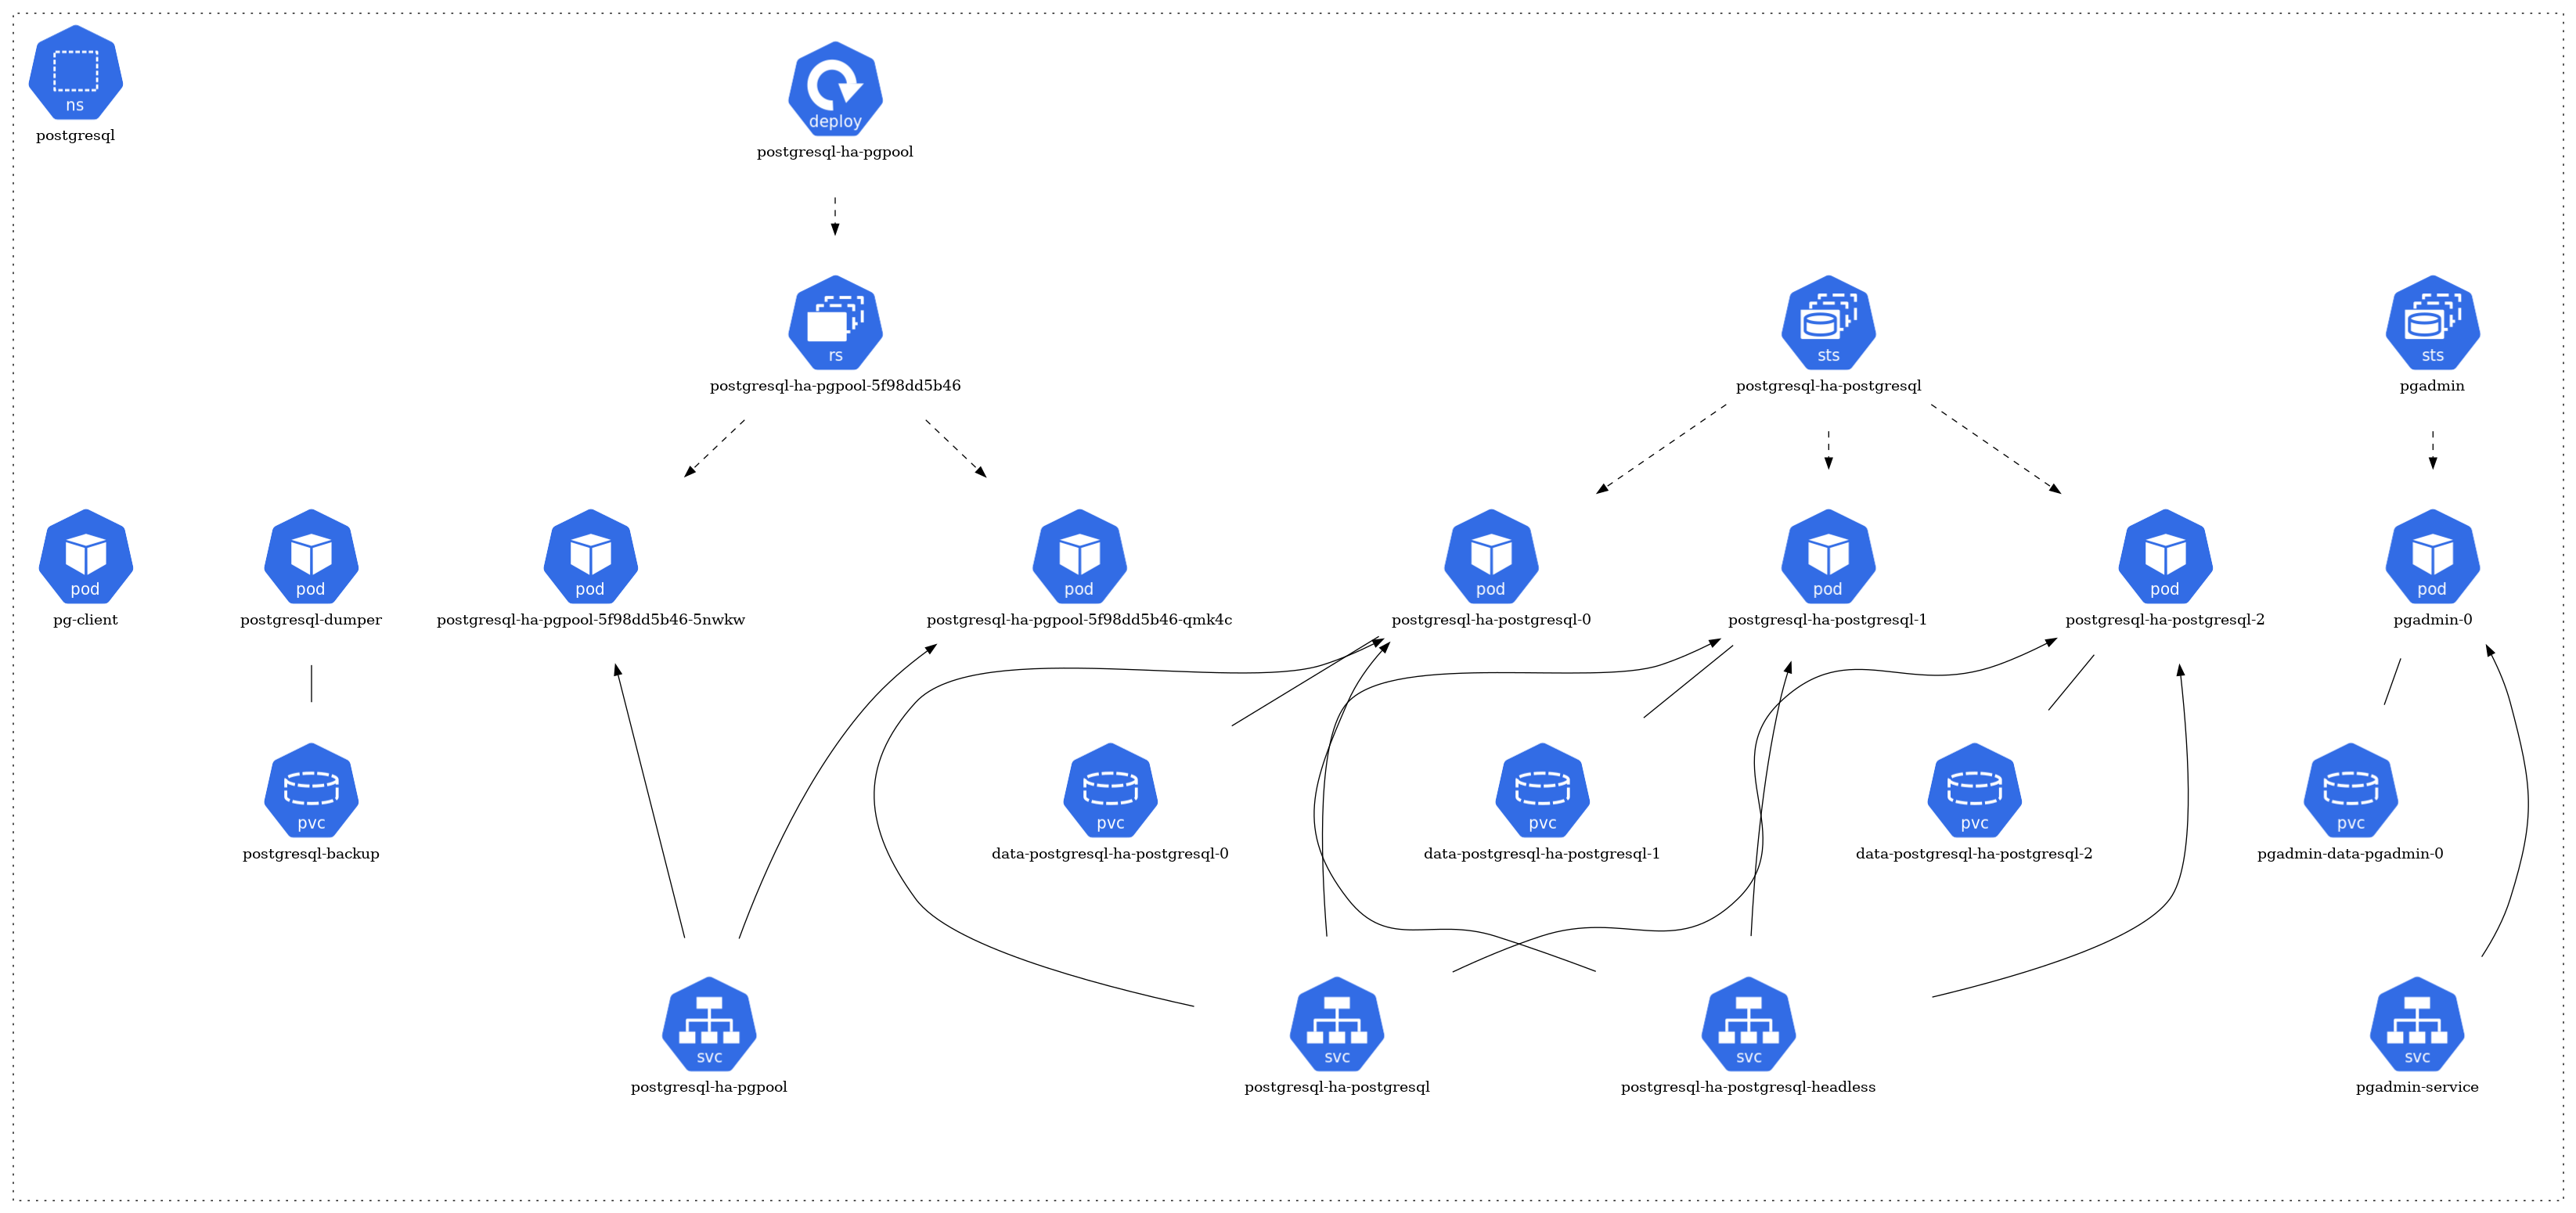
\includegraphics[width=1.0\textwidth,angle=00]{assets/f37.png}
\caption{HA PostgreSQL Workloads}
\label{fig:f37}
\end{figure}

This configuration ensures that one PostgreSQL instance always serves as the primary node that accepts all writes and updates, while the other instances act as standby nodes that replicate data from the primary node. 

\subsubsection{Replicated Redis }

Redis is an in-memory data structure store used as a database, cache, and message broker. 
\begin{itemize}[label={--}]
\item In a similar fashion to HA postgresql, deploying a replicated Redis cluster on Kubernetes involves: 
\item using a Kubernetes StatefulSet to deploy multiple Redis instances in a replicated configuration, 
\item configuring Redis replication for data synchronization, 
\item using a Kubernetes Service to provide a stable endpoint for accessing the Redis cluster, 
\item and using a Kubernetes PVC to ensure data persistence. 
\end{itemize}
With this setup, you can have a highly available and scalable Redis database infrastructure for your containerized applications. 

The resulting setup is illustrated by the following figure: 

\begin{figure}[H]\centering
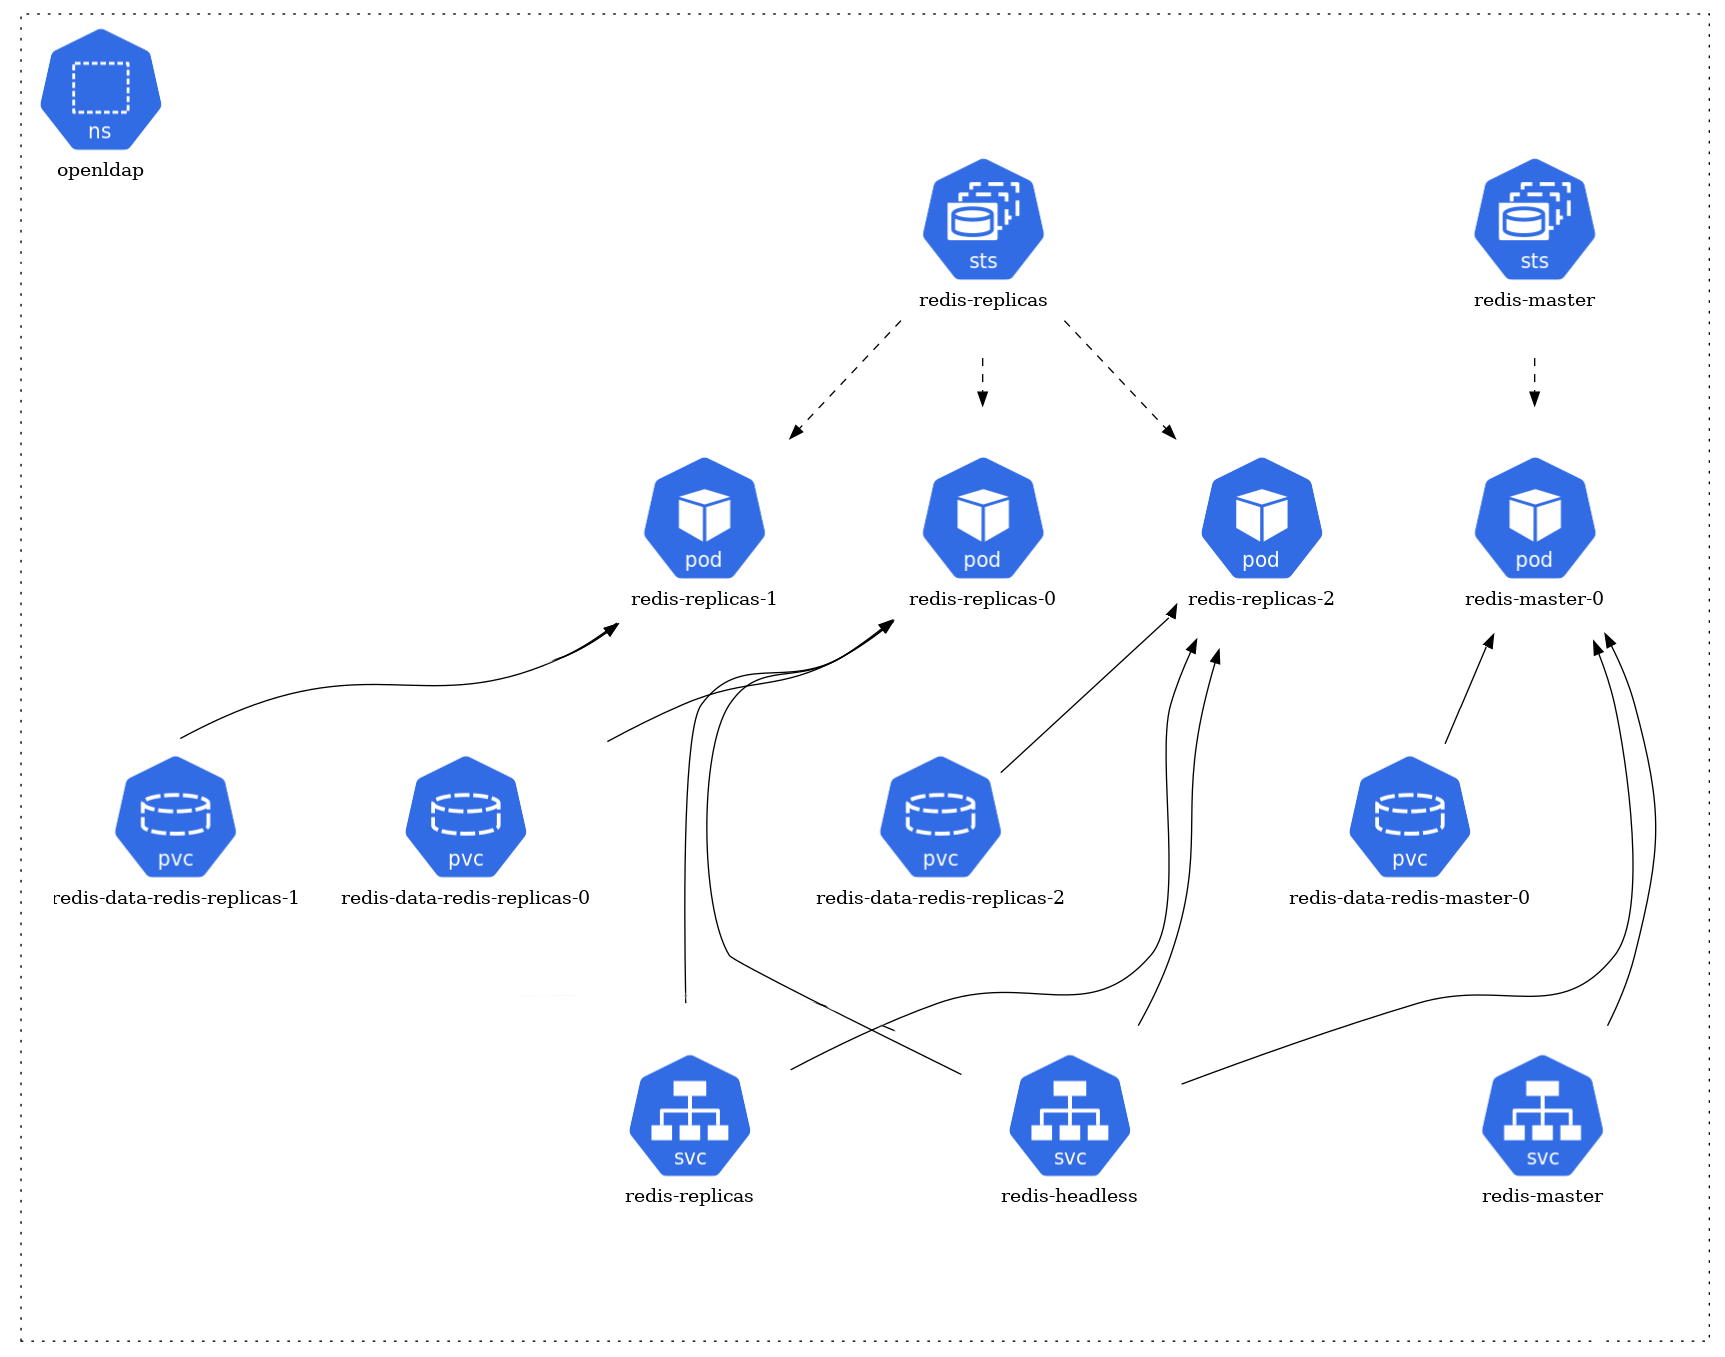
\includegraphics[width=1.0\textwidth,angle=00]{assets/f38.png}
\caption{Redis Setup }
\label{fig:Redis Setup}
\end{figure}

\subsection{Artifact registry }

In a CI/CD platform, having an artifact registry is necessary to allows users to store, sign, and scan container images for vulnerabilities. This has been tackled using harbor. It also provides features such as user management, access control, and replication for distributing images across multiple registry instances. 

\subsubsection{diagram for deploying the artifact registry}

\begin{figure}[H]\centering
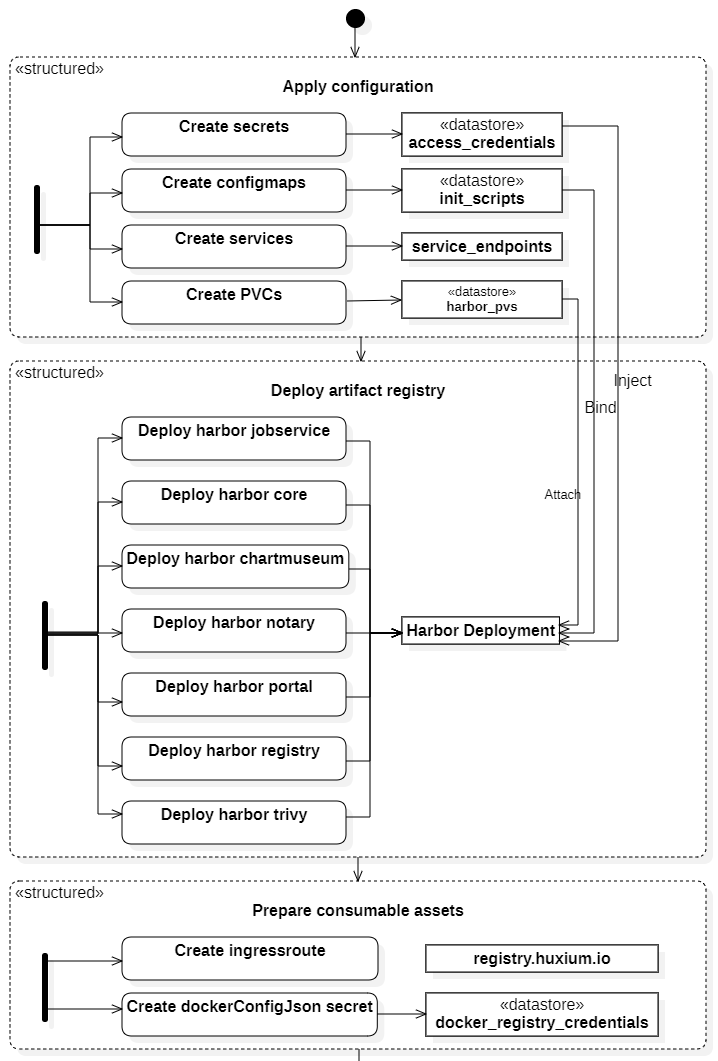
\includegraphics[width=0.9\textwidth,angle=00]{assets/f39.png}
\caption{diagram for deploying the artifact registry }
\label{fig:diagram for deploying the artifact registry}
\end{figure}

\subsubsection{Deploying the artifact registry }

Deploying Harbor on Kubernetes involves creating and configuring the necessary Kubernetes resources. 

Here are the high-level steps for deploying Harbor on Kubernetes: 
\begin{enumerate}
\item Create a Kubernetes secret for the Harbor admin password 
\item Create configmaps for the deployment to use the deployed database services (Redis for cache storage and postgresql for metadata storage). 
\item Create persistent volume claims (PVC) for data storage. 
\item Create a Kubernetes deployment for each Harbor service. 
\item Create ClusterIP services for internal access. 
\item Create ingressroutes for external access through https. 
\item Create a dockerConfigJson secret to use for pulling images from private projects in harbor. 
\end{enumerate}

The following is an illustration on the deployed services: 
\begin{figure}[H]\centering
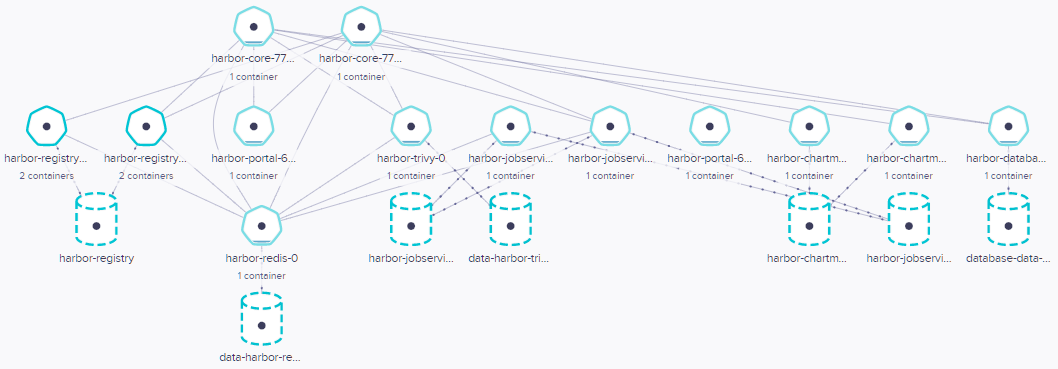
\includegraphics[width=1.0\textwidth,angle=00]{assets/f40.png}
\caption{deployed services}
\label{fig:Deployed services}
\end{figure}

\subsection{Code quality gate}

Software development is a complex and iterative process, and it is important to have tools that can help identify and address issues in the codebase as early as possible. 

SonarQube is a powerful code quality and security analysis tool that can be integrated with Kubernetes to help ensure that the code running in your Kubernetes environment is of high quality and secure. 

\subsubsection{Activity diagram for deploying the code quality gate}

\begin{figure}[H]\centering
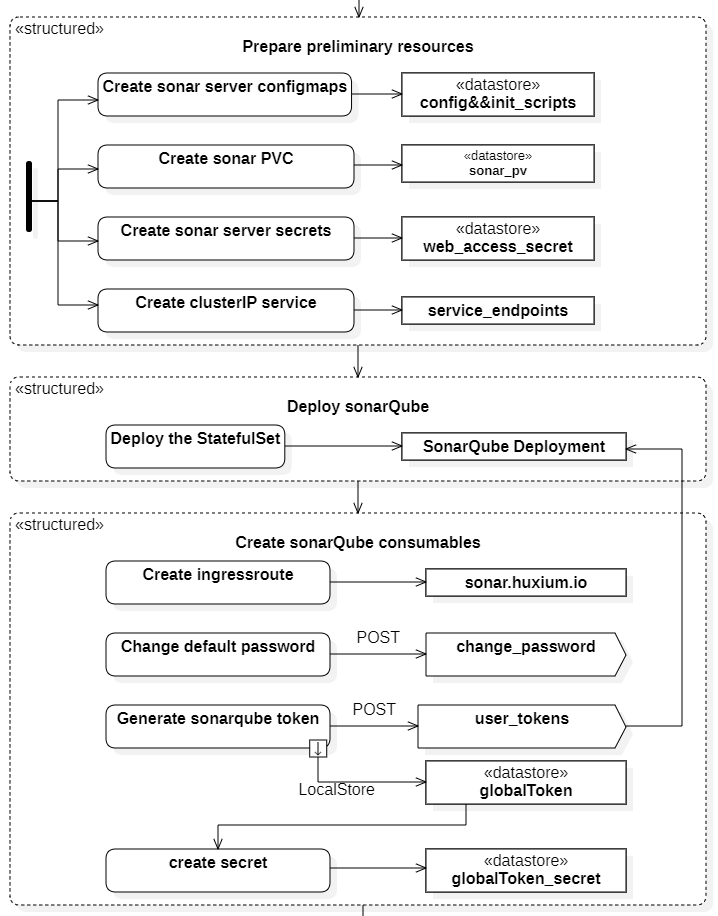
\includegraphics[width=1.0\textwidth,angle=00]{assets/f41.png}
\caption{Activity diagram for deploying the code quality gate}
\label{fig:Activity diagram for deploying the code quality gate}
\end{figure}

\subsubsection{Deploying the code quality gate }

Deploying a SonarQube cluster on Kubernetes involves creating and configuring the necessary Kubernetes resources. 

Here are the high-level steps: 
\begin{enumerate}
\item Create a Kubernetes secret for configuring web access 
\item Create configmaps to configure the deployment to use the deployed database services (Redis for cache storage and postgresql for metadata storage). 
\item Create persistent volume claims (PVC) for data storage. 
\item Create a Kubernetes StatefulSet for deploying the cluster pods. 
\item Create ClusterIP services for internal access. 
\item Create ingressroutes for external access through https. 
\item Using the “ansible.builtin.uri” module, a POST request is sent to the SonarQube api to change the default admin password and generate a global token to be used by the cicd orchestrator. This token is then stored in a Kubernetes secret: 
\end{enumerate}

\begin{figure}[H]\centering
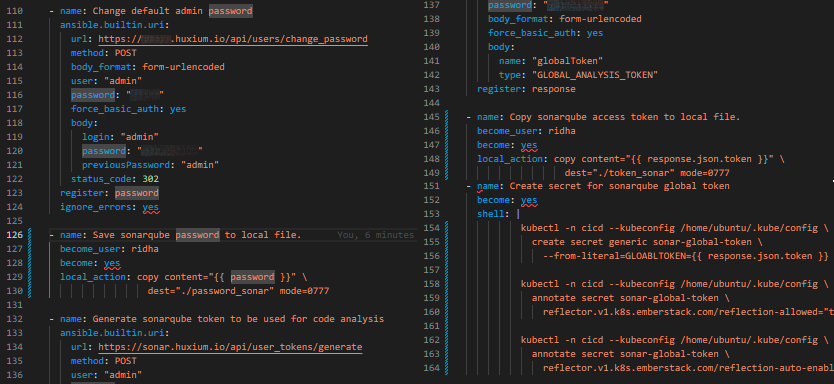
\includegraphics[width=1.0\textwidth,angle=00]{assets/f42.png}
% \caption{Figure 42 }
% \label{fig:f42}
\end{figure}

\subsection{CD/CD controller }

For the continuous deployment and continuous deployment aspect of our pipelines, we chose to use ArgoCD. 

Our CD/CD controller is configured to feature the following characteristics:  
\begin{itemize}[label={--}]
\item GitOps-based approach: we are useing a GitOps-based approach to CD/CD. This means that all configuration changes and deployments are done through GitLAB, our SCM of choice. 
\item Automated deployments: applications are deployed based on changes to their respective Git repositories. This eliminates the need for manual deployments and ensures that our applications are always up-to-date. 
\item Declarative configuration management: we use a declarative configuration management approach to CD/CD. This means that we define the desired state of our Kubernetes workloads in a configuration file, and ArgoCD ensures that the actual state matches the desired state. 
\end{itemize}

Furthermore, argoCD provides a web-based interface to view the deployed workloads and their sync states: 

\begin{figure}[H]\centering
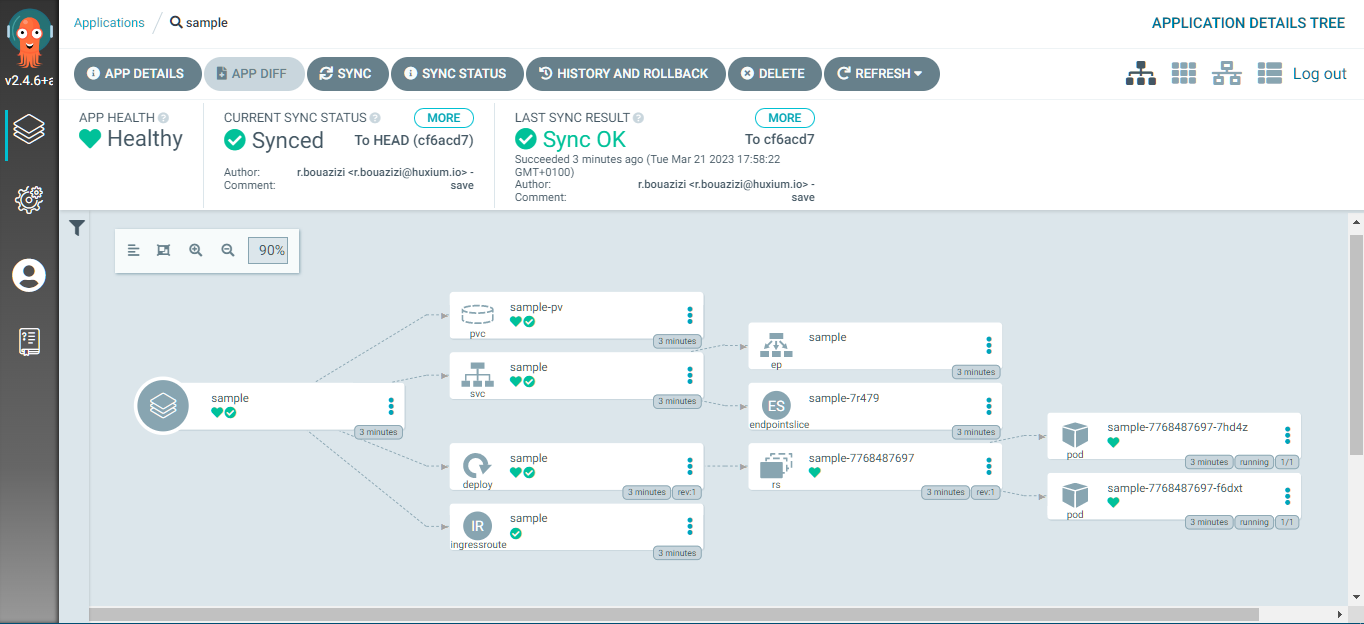
\includegraphics[width=1.0\textwidth,angle=00]{assets/f43.png}
\caption{ AgroCD interface }
\label{fig:AgroCD interface}
\end{figure}
 

\subsection{CI/CD orchestrator }

Jenkins, our CI/CD orchestrator of choice, provides a wide range of features and plugins that can be used to automate various stages of the software development process, including building, testing, and deploying applications. The following is the activity diagram for deploying it. 

 
\subsubsection{UML Design: Activity diagram for deploying the CI/CD orchestrator components : }

\begin{figure}[H]\centering
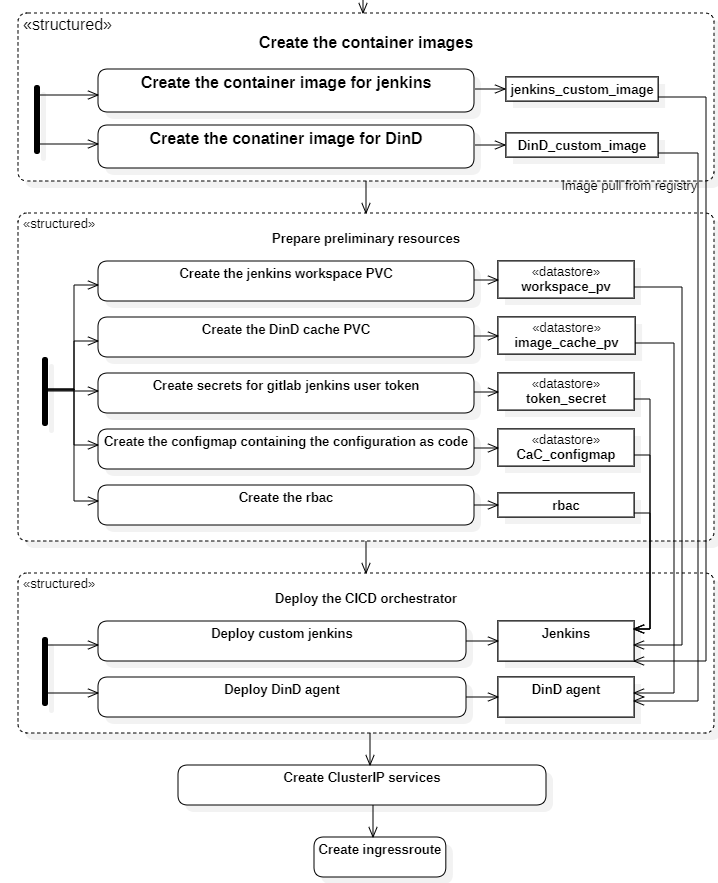
\includegraphics[width=1.0\textwidth,angle=00]{assets/f44.png}
\caption{Activity diagram for deploying the CI/CD orchestrator components}
\label{fig:Activity diagram for deploying the CI/CD orchestrator components}
\end{figure}
 
\subsubsection{The personalized jenkins container image: }

As a CI/CD orchestrator, Jenkins acts as a central hub that integrates with various tools and systems involved in the software development pipeline. The container image for this deployment is prepackaged with the initial configuration of the various cloud providers we are using, the server tokens and access credentials. Thus, the container image is ready to go as soon as it is deployed. The resulting Dockefile is as follows : 

\begin{listing}[H]
    \inputminted{Dockerfile}{codeListing/jenkins_Dockerfile}
    \caption{Jenkins Dockerfile}
    \label{lst:Jenkins Dockerfile}
\end{listing}

\subsubsection{The Docker in Docker container image: }

For building container images for the application under development, a technique that allows running Docker commands within a Docker container is used. To enable DinD, a Docker image is created with Docker installed inside it. Furthermore, authentication to the private registry is streamlined into the container execution. The following is the resulting Dockerfile: 

\begin{listing}[H]
    \inputminted{Dockerfile}{codeListing/dind-Dockerfile}
    \caption{Dind Dockerfile}
    \label{lst:Dind Dockerfile}
\end{listing}

\section*{Conclusion}
In conclusion, deploying a CI/CD platform in Kubernetes can be a challenging task, but it provides a powerful and scalable solution for continuous integration and deployment. 

By leveraging tools like Jenkins, Docker in Docker, ArgoCD, Harbor, and SonarQUBE, we can streamline the development process and achieve faster, more reliable deployments. This setup allows us to build and test code continuously, scan code for potential security vulnerabilities, and deploy applications quickly and efficiently. 

With the right tools and techniques, we created a comprehensive and effective CI/CD platform that enables us to deliver high-quality software at a faster pace.